% ============================================================
%  Tensor DEIM — Progress Update
%  Compile with: pdflatex slides_tdeim.tex  (run twice)
%  Requires metropolis theme: tlmgr install beamer-theme-metropolis
%  Figures must be in the same directory as this .tex file.
% ============================================================
\documentclass[aspectratio=169, 11pt]{beamer}

\usetheme{metropolis}

% ── packages ────────────────────────────────────────────────
\usepackage{booktabs}
\usepackage{colortbl}
\usepackage{amsmath, amssymb}
\usepackage{graphicx}
\usepackage{xcolor}
\usepackage{tikz}
\usepackage[protrusion=true, expansion=false]{microtype}
\usepackage[T1]{fontenc}
\usetikzlibrary{arrows.meta}

\graphicspath{{./}}

% ── colour palette ──────────────────────────────────────────
\definecolor{cnavy}{HTML}{0D2137}
\definecolor{cteal}{HTML}{1A6B8A}
\definecolor{cice}{HTML}{D6EBF5}
\definecolor{camber}{HTML}{F0A500}
\definecolor{cgreen}{HTML}{1D8A5E}
\definecolor{cred}{HTML}{C0392B}
\definecolor{cmuted}{HTML}{5A7385}

% ── metropolis overrides ────────────────────────────────────
\setbeamercolor{normal text}{fg=cnavy, bg=white}
\setbeamercolor{frametitle}{bg=cnavy, fg=white}
\setbeamercolor{title separator}{fg=cteal}
\setbeamercolor{progress bar}{fg=cteal, bg=cice}
\setbeamercolor{alerted text}{fg=camber}
\setbeamercolor{block title}{bg=cice, fg=cnavy}
\setbeamercolor{block body}{bg=cice!40, fg=cnavy}
\setbeamercolor{itemize item}{fg=cteal}
\setbeamercolor{itemize subitem}{fg=cmuted}
\setbeamercolor{enumerate item}{fg=cteal}
\setbeamerfont{frametitle}{size=\large, series=\bfseries}
\setbeamerfont{block title}{series=\bfseries, size=\small}
\setbeamerfont{block body}{size=\small}

% ── macros ───────────────────────────────────────────────────
\newcommand{\epod}{\varepsilon_{\mathrm{POD}}}
\newcommand{\Phimat}{\boldsymbol{\Phi}}
\newcommand{\tightarrow}{%
  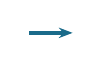
\begin{tikzpicture}[baseline=-0.5ex]
    \draw[-{Stealth[length=5pt]}, line width=1.2pt, color=cteal] (0,0)--(0.55,0);
  \end{tikzpicture}}

% ── title info ───────────────────────────────────────────────
\title{Tensor DEIM}
\subtitle{for Lossy Compression of 3D Scientific Data}
\author{Jessie Chen}
\institute{Argonne National Laboratory}
\date{July 2026}

% ============================================================
\begin{document}
% ============================================================

% ── SLIDE 1: Title ──────────────────────────────────────────
\maketitle

% ── SLIDE 2: Dataset ────────────────────────────────────────
\begin{frame}{Dataset: ISABEL Hurricane Simulation}
\begin{columns}[T]

\begin{column}{0.50\textwidth}
  \textcolor{cteal}{\textbf{Structure at a glance}}
  \begin{itemize}\setlength\itemsep{0.3em}\small
    \item 100 vertical levels (surface $\to$ upper atmosphere)
    \item $500 \times 500$ spatial grid (lat $\times$ lon) per level
    \item $\approx 25$\,M floating-point values per field
    \item Fields: U, V, W wind + pressure, temperature, \ldots
    \item Goal: store ${<}1\%$ of data, reconstruct with ${<}1\%$ error
  \end{itemize}
\end{column}

\begin{column}{0.46\textwidth}
  \begin{block}{}
    \textcolor{cteal}{\textbf{25\,M}} \hfill
    \scriptsize values/field \enspace($100\!\times\!500\!\times\!500$)
  \end{block}\vspace{0.12em}
  \begin{block}{}
    \textcolor{cteal}{\textbf{100$\times$}} \hfill
    \scriptsize compression target
  \end{block}\vspace{0.12em}
  \begin{block}{}
    \textcolor{cteal}{\textbf{$\leq 1\%$}} \hfill
    \scriptsize error tolerance
  \end{block}\vspace{0.12em}
  \begin{block}{}
    \textcolor{cteal}{\textbf{1\,:\,278.89}} \\[-0.1em]
    \scriptsize T-DEIM compression ratio
    (k\,=\,100 sensors vs 27{,}889 pts/level)
  \end{block}
\end{column}

\end{columns}
\end{frame}

% ── SLIDE 3: Why T-DEIM? ────────────────────────────────────
\begin{frame}{Why Tensor DEIM?}
\begin{columns}[T]

\begin{column}{0.48\textwidth}
  \begingroup
  \setbeamercolor{block title}{bg=cred!15, fg=cred}
  \setbeamercolor{block body}{bg=cred!5, fg=cnavy}
  \begin{block}{GP / Kriging approach}
    \begin{itemize}\setlength\itemsep{0.3em}
      \item Slice-by-slice: each of 100 levels solved independently
      \item Full $n{\times}n$ covariance matrix $\to$ memory wall at fine grids
      \item No exploitation of vertical correlations
      \item Reconstruction: one 2D slice at a time
    \end{itemize}
  \end{block}
  \endgroup
\end{column}

\begin{column}{0.48\textwidth}
  \begingroup
  \setbeamercolor{block title}{bg=cgreen!15, fg=cgreen}
  \setbeamercolor{block body}{bg=cgreen!5, fg=cnavy}
  \begin{block}{T-DEIM approach}
    \begin{itemize}\setlength\itemsep{0.3em}
      \item Treats the full 3D field as one object
      \item SVD of mode-1 unfolding $\to$ global low-rank structure
      \item $k$ sensors anywhere in the 3D volume
      \item One solve $\to$ all 100 levels reconstructed at once
    \end{itemize}
  \end{block}
  \endgroup
\end{column}

\end{columns}
\end{frame}

% ── SLIDE 4: Algorithm ──────────────────────────────────────
\begin{frame}{T-DEIM Algorithm — Step by Step}
\small
\begin{enumerate}\setlength\itemsep{0.35em}
  \item \textbf{Mode-1 unfolding:} reshape 3D field $F$ ($n_L \!\times\! n_Y \!\times\! n_Z$)
        $\to$ matrix $A$ ($n_L \!\times\! n$), \; $n = n_Y \cdot n_Z$

  \item \textbf{Thin SVD:} $A = U\Sigma V^T$. \quad
        $U$: level modes ($n_L \!\times\! r$); \;
        $V^T$: spatial modes ($r \!\times\! n$)

  \item \textbf{Adaptive rank $k$:} smallest $k$ s.t.\
        $\epod \leq \texttt{ERROR\_TOL}$

  \item \textbf{Rank-1 3D modes:}
        $\varphi_j = \mathrm{flatten}(u_j \otimes v_j^T)$, shape $(n_L \cdot n,)$.
        Columns of $\Phimat$ are orthonormal.

  \item \textbf{Q-DEIM placement:} QR column-pivoting on $\Phimat^T$
        gives $p = k + \texttt{OVERSAMPLE}$ sensor indices in the 3D volume

  \item \textbf{Least-squares solve:} observe $y_\mathrm{obs}$ at $p$ sensors;
        solve $\Phimat[\mathrm{sensors},:]\,c \approx y_\mathrm{obs}$
        via \texttt{lstsq} \;($p > k$)

  \item \textbf{Full reconstruction:}
        $\hat{F} = \mathrm{reshape}(\Phimat c,\; n_L \!\times\! n_Y \!\times\! n_Z)$.
        All 100 levels from one solve.
\end{enumerate}
\end{frame}

% ── SLIDE 5: Mode-1 Unfolding ────────────────────────────────
\begin{frame}{Mode-1 Unfolding — How T-DEIM Uses the 3D Tensor}

\begin{columns}[c]
\begin{column}{0.28\textwidth}
  \begin{block}{3D Tensor $F$}
    \scriptsize Shape: $100\!\times\!167\!\times\!167$\\
    $= 2.8$\,M values/snapshot\\[0.2em]
    Each `slab' = one altitude level
  \end{block}
\end{column}
\begin{column}{0.05\textwidth}\centering\tightarrow\end{column}
\begin{column}{0.27\textwidth}
  \begin{block}{Matrix $A$}
    \scriptsize Shape: $100\!\times\!27{,}889$\\[0.2em]
    Each ROW = one flattened level ($n_Y \!\times\! n_Z$ pixels)
  \end{block}
\end{column}
\begin{column}{0.05\textwidth}\centering\tightarrow\end{column}
\begin{column}{0.30\textwidth}
  \begin{block}{SVD Factors}
    \scriptsize
    $U_L$: $100\!\times\!k$ vertical profiles\\
    $\Sigma$: $k\!\times\!k$ singular values\\
    $V^T$: $k\!\times\!n$ spatial patterns\\[0.2em]
    $\varphi_j = \mathrm{outer}(U_L[:,j],\,V^T[j,:])$
  \end{block}
\end{column}
\end{columns}

\vspace{0.4em}

\begin{columns}[T]
\begin{column}{0.48\textwidth}
  \begingroup
  \setbeamercolor{block title}{bg=cred!15, fg=cred}
  \setbeamercolor{block body}{bg=cred!5, fg=cnavy}
  \begin{block}{2D Q-DEIM — slice-by-slice}
    \scriptsize
    \begin{itemize}\setlength\itemsep{0.15em}
      \item Uses only $V^T$ (right singular vectors = spatial modes)
      \item Sensors fixed in one (lat, lon) plane — same $(y,z)$ every level
      \item 100 independent $k\!\times\!k$ solves (one per level)
      \item Does NOT exploit how the field changes with altitude
    \end{itemize}
  \end{block}
  \endgroup
\end{column}
\begin{column}{0.48\textwidth}
  \begingroup
  \setbeamercolor{block title}{bg=cgreen!15, fg=cgreen}
  \setbeamercolor{block body}{bg=cgreen!5, fg=cnavy}
  \begin{block}{T-DEIM — 3D global solve}
    \scriptsize
    \begin{itemize}\setlength\itemsep{0.15em}
      \item Uses $U_L \otimes V^T$ — rank-1 modes spanning all 3D
      \item Sensors anywhere in volume: each has its own $(lv, y, z)$
      \item ONE global solve $\to$ all 100 levels at once
      \item $U_L$ encodes vertical variation $\to$ sensors go to most informative levels
    \end{itemize}
  \end{block}
  \endgroup
\end{column}
\end{columns}

\end{frame}

% ── SLIDE 6: Error bound ─────────────────────────────────────
\begin{frame}{Adaptive $k$ — Drmač \& Gugercin Error Bound}

\vspace{-0.2em}
\begingroup
\setbeamercolor{block title}{bg=cice, fg=cnavy}
\setbeamercolor{block body}{bg=cice!60, fg=cnavy}
\begin{block}{Theorem \normalfont\footnotesize(Drmač \& Gugercin 2016, SIAM J.\ Sci.\ Comput.\ 38(2):A631–A648)}
\vspace{-0.4em}
\[
\|f - P_{\mathrm{DEIM}} f\|
\;\leq\;
\bigl(1 + \|(\Phimat^T[s,:])^{-1}\|_2\bigr)
\;\times\;
\|(I - \Phimat\Phimat^T)\,f\|
\]
\vspace{-0.6em}
\end{block}
\endgroup

\vspace{0.15em}
\begin{columns}[T]
\begin{column}{0.48\textwidth}
  \begin{block}{Term 1 — $\Lambda$ (Lebesgue constant)}
    \scriptsize
    $\Lambda = \|(\Phimat^T[s,:])^{-1}\|_2 = 1/\sigma_{\min}(\Phimat[s,:])$

    \smallskip
    Q-DEIM (QR pivoting) removes the exponential factor in the original DEIM bound.
    Oversampling $p = k+10$ improves $\sigma_{\min}$. Typically $\Lambda \approx 2$–$5$.
  \end{block}
\end{column}
\begin{column}{0.48\textwidth}
  \begin{block}{Term 2 — $\epod$ (truncation error)}
    \scriptsize
    $\displaystyle
      \epod = \frac{\|(I-\Phimat\Phimat^T)f\|}{\|f\|}
             = \frac{\sqrt{\sum_{i>k}\sigma_i^2}}{\|A\|_F}$

    \smallskip
    Read from the singular value spectrum.
    Set by \texttt{ERROR\_TOL}: add modes until $\epod \leq \texttt{tol}$.
  \end{block}
\end{column}
\end{columns}

\vspace{0.15em}
{\small\textcolor{camber}{\textbf{This work:}}
\texttt{GUARANTEE\_MODE=`trunc'} selects smallest $k$ with $\epod \leq 1\%$.
The a priori bound $(1\!+\!\Lambda)\cdot\epod$ can be $\gg 1\%$ (conservative worst-case);
empirical errors are orders of magnitude smaller.}

\end{frame}

% ── SLIDE 7: Error control modes ────────────────────────────
\begin{frame}{Error Control Modes — \texttt{GUARANTEE\_MODE}}

\vspace{0.05em}
{\small Two parameters: \texttt{ERROR\_TOL} (relative) and \texttt{ABS\_TOL} (absolute, m/s).}

\vspace{0.15em}
\scriptsize
\renewcommand{\arraystretch}{1.05}
\begin{tabular}{p{1.6cm}p{3.2cm}p{4.2cm}p{2.5cm}}
\toprule
\rowcolor{cnavy}
\textcolor{white}{\textbf{Mode}} &
\textcolor{white}{\textbf{$k$ chosen so that}} &
\textcolor{white}{\textbf{Guarantee type}} &
\textcolor{white}{\textbf{Parameter}} \\
\midrule
\texttt{'trunc'}
  & $\epod \leq \texttt{ERROR\_TOL}$
  & POD truncation bound. Fast; no sensor quality check.
  & \texttt{ERROR\_TOL} \\
\rowcolor{cice!50}
\texttt{'apriori'}
  & $(1+\Lambda)\cdot\epod \leq \texttt{ERROR\_TOL}$
  & Full Drmač a priori bound. Raises $k$ until $\Lambda$ is small enough. Conservative but rigorous.
  & \texttt{ERROR\_TOL} \\
\texttt{'abs'}
  & $\mathrm{RMSE} \leq \texttt{ABS\_TOL}$
  & Absolute field-unit bound (m/s). Analogous to SZ-1.4 pointwise tolerance; relative errors vary by level.
  & \texttt{ABS\_TOL} \\
\rowcolor{cice!50}
\texttt{None}
  & Same as \texttt{'trunc'}
  & No guarantee label in output. Useful for exploration.
  & \texttt{ERROR\_TOL} \\
\bottomrule
\end{tabular}

\vspace{0.3em}
{\scriptsize\textcolor{cmuted}{%
  \texttt{ERROR\_TOL} is the single relative tolerance for all modes (\texttt{'trunc'}, \texttt{'apriori'}, \texttt{None}).
  \texttt{ABS\_TOL} (m/s) is only consulted by \texttt{'abs'} mode.
  A priori bound is conservative; empirical errors are typically $\ll$ target.}}

\end{frame}

% ── SLIDE 8: Computational cost ──────────────────────────────
\begin{frame}{Computational Cost Comparison}

{\scriptsize\textit{%
  SZ-1.4: Tao et al.\ (2017), IPDPS.\ ISABEL $100\!\times\!500\!\times\!500$.
  DEIM methods at DOWNSAMPLE\,=\,3: $n=27{,}889$ pts/level, $k\approx30$–80.}}

\vspace{0.05em}
{\hfuzz=20pt\scriptsize
\renewcommand{\arraystretch}{1.1}
\begin{tabular}{p{1.6cm}p{1.9cm}p{3.2cm}p{3.8cm}}
\toprule
\rowcolor{cnavy}
\textcolor{white}{\textbf{Phase}} &
\textcolor{white}{\textbf{SZ-1.4}} &
\textcolor{white}{\textbf{2D Q-DEIM\newline(layer-by-layer)}} &
\textcolor{white}{\textbf{T-DEIM\newline(3D global solve)}} \\
\midrule
Offline
  & None
  & SVD: $O(n\, n_{\rm tr}^2)$\newline QR: $O(nk^2)$
  & SVD: $O(n_L^2 n)$\newline QR: $O(nk^2)$ \\
\rowcolor{cred!8}
\textbf{Encode}
  & \textcolor{cred}{\textbf{$O(N)$}}\newline
    \textcolor{cred}{pred+quant,}\newline
    \textcolor{cred}{Huffman}
  & \textcolor{cgreen}{\textbf{$O(k)$ reads/level}}\newline
    \textcolor{cgreen}{100 indep.\ solves}
  & \textcolor{cgreen}{\textbf{$O(k)$ reads total}}\newline
    \textcolor{cgreen}{one solve $\to$ all levels} \\
Decode
  & $O(N)$
  & $O(nk)$/level $\times\,100$
  & $O(Nk)$ matvec \\
Sensors
  & —
  & Same $(y,z)$ for all levels
  & Free $(lv,y,z)$ in 3D \\
Error
  & Pointwise abs.
  & Per-level $\epod$
  & Global Frobenius $\epod$ \\
Full-res?
  & Yes
  & Yes — SVD at $n\!=\!250\text{k}$
  & rSVD needed \\
\bottomrule
\end{tabular}}

\end{frame}

% ── SLIDE 8: Sensor distribution ─────────────────────────────
\begin{frame}{Where Does T-DEIM Place Its Sensors?}
\vspace{-0.3em}
\begin{center}
  \includegraphics[width=0.88\textwidth]{tdeim_sensor_distribution.png}
\end{center}
\vspace{-0.5em}
{\scriptsize\textcolor{cmuted}{%
  Left: sensors cluster on levels where vertical wind structure is most variable.
  Right: spatial (lat, lon) scatter.
  Error criterion: $\epod \leq 1\%$, \texttt{trunc} mode.}}
\end{frame}

% ── SLIDE 9: Per-level error histogram ───────────────────────
\begin{frame}{Reconstruction Error — All 100 Altitude Levels}
\vspace{-0.3em}
\begin{center}
  \includegraphics[width=0.93\textwidth]{tdeim_level_errors.png}
\end{center}
\vspace{-0.4em}
{\scriptsize\textcolor{cmuted}{%
  Green: within 1\% guarantee.
  Grey: near-zero levels (wind $\approx 0$) excluded.
  Log scale — empirical errors are orders of magnitude below the 1\% target.
  Error criterion: $\epod \leq 1\%$, \texttt{trunc} mode.}}
\end{frame}

% ── SLIDE 10: T-DEIM vs 2D Q-DEIM comparison ────────────────
\begin{frame}{T-DEIM vs 2D Q-DEIM — Same Sensors, Better Accuracy}
\vspace{-0.1em}
\begin{center}
  \includegraphics[height=0.65\textheight]{tdeim_comparison.png}
\end{center}
\vspace{-0.4em}
{\scriptsize\textcolor{cmuted}{%
  $k=41$ sensors, CLOUD field, DOWNSAMPLE=3. T-DEIM: 5.56\% error vs 10.59\% (2D Q-DEIM).
  T-DEIM sensors range freely across all altitudes; 2D sensors fixed to one (lat,\,lon) plane.
  \textit{(Regenerate at consistent $k$ with slide 9 before final version.)}}}
\end{frame}

% ── SLIDE 11: Path to <1% ────────────────────────────────────
\begin{frame}{Path to ${<}1\%$ Reconstruction Error}
\begin{columns}[T]

\begin{column}{0.32\textwidth}
  \begin{block}{\textcircled{\scriptsize 1}\; Lower \texttt{ERROR\_TOL}}
    \small \texttt{ERROR\_TOL = 1e-3} forces more modes $k$,
    directly shrinking $\epod$. Most direct lever.
  \end{block}\vspace{0.3em}
  \begin{block}{\textcircled{\scriptsize 4}\; Randomized T-DEIM}
    \small Replace dense SVD with rSVD + randomized sensor selection.
    Enables DOWNSAMPLE\,=\,1 without memory wall.
  \end{block}
\end{column}

\begin{column}{0.32\textwidth}
  \begin{block}{\textcircled{\scriptsize 2}\; Oversampling \emph{(added)}}
    \small $p = k + 10$ sensors $\to$ overdetermined least-squares.
    Reduces Lebesgue constant $\Lambda$ and noise sensitivity.
  \end{block}\vspace{0.3em}
  \begin{block}{\textcircled{\scriptsize 5}\; Per-level normalization}
    \small Current z-score is global.
    Per-level normalization tightens basis for outlier altitude levels.
  \end{block}
\end{column}

\begin{column}{0.32\textwidth}
  \begin{block}{\textcircled{\scriptsize 3}\; Multi-snapshot basis}
    \small Build $\Phimat$ from several timesteps.
    Richer training $\to$ lower $\epod$ for any given $k$.
  \end{block}\vspace{0.3em}
  \begin{block}{\textcircled{\scriptsize 6}\; Joint multi-field basis}
    \small Combine U, V, W into one tall $A$.
    Cross-field correlations may yield a lower-rank basis.
  \end{block}
\end{column}

\end{columns}
\end{frame}

% ── SLIDE 12: Next steps ──────────────────────────────────────
\begin{frame}[standout]
  \large\textbf{Next Steps}\\[0.4em]
  \normalsize\textcolor{cteal!70!white}{%
    T-DEIM $\;\to\;$ Randomized T-DEIM $\;\to\;$ Full-resolution evaluation}

  \vspace{0.8em}
  \begin{itemize}\setlength\itemsep{0.45em}
    \item Tune \texttt{ERROR\_TOL} to push reconstruction error below 1\% across all levels
    \item Add randomized SVD (rSVD) — enables full-resolution (DOWNSAMPLE\,=\,1) runs
    \item Implement randomized Q-DEIM sensor selection (Saibaba 2020)
    \item Extend to V, W wind fields and pressure; evaluate cross-field compression
  \end{itemize}
\end{frame}

% ============================================================
\end{document}
